\documentclass[10pt, letterpaper]{article}

% Packages:
\usepackage[
  ignoreheadfoot, % set margins without considering header and footer
  top=0.75in, % seperation between body and page edge from the top
  bottom=0.75in, % seperation between body and page edge from the bottom
  left=0.75in, % seperation between body and page edge from the left
  right=0.75in, % seperation between body and page edge from the right
  % footskip=1.0 cm, % seperation between body and footer
  % showframe % for debugging
]{geometry} % for adjusting page geometry
\usepackage{titlesec} % for customizing section titles
\usepackage{tabularx} % for making tables with fixed width columns
\usepackage{array} % tabularx requires this
\usepackage[dvipsnames]{xcolor} % for coloring text
\definecolor{primaryColor}{RGB}{0, 0, 0} % define primary color
\usepackage{enumitem} % for customizing lists
\usepackage{fontawesome5} % for using icons
\usepackage{amsmath} % for math
\usepackage[
  pdftitle={Rohan's CV},
  pdfauthor={Mahmud Abdul Aziz Rohan},
  pdfcreator={LaTeX with RenderCV},
  colorlinks=true,
  urlcolor=primaryColor
]{hyperref} % for links, metadata and bookmarks
\usepackage[pscoord]{eso-pic} % for floating text on the page
\usepackage{calc} % for calculating lengths
\usepackage{bookmark} % for bookmarks
% \usepackage{lastpage} % for getting the total number of pages
\usepackage{changepage} % for one column entries (adjustwidth environment)
\usepackage{paracol} % for two and three column entries
\usepackage{ifthen} % for conditional statements
\usepackage{needspace} % for avoiding page brake right after the section title
\usepackage{iftex} % check if engine is pdflatex, xetex or luatex
\usepackage{ragged2e}

\usepackage{graphicx}
\usepackage{tikz}
\usetikzlibrary{calc}

% Ensure that generate pdf is machine readable/ATS parsable:
\ifPDFTeX
\input{glyphtounicode}
\pdfgentounicode=1
\usepackage[T1]{fontenc}
\usepackage[utf8]{inputenc}
\usepackage{lmodern}
\fi

\usepackage{fontspec}
% \setmainfont{XCharter}[
%     Extension = .otf,
%     UprightFont = *-Regular,
%     BoldFont = *-Bold,
%     ItalicFont = *-Italic,
%     BoldItalicFont = *-BoldItalic,
% ]

% Some settings:
\raggedright
\AtBeginEnvironment{adjustwidth}{\partopsep0pt} % remove space before
% adjustwidth environment
\pagestyle{empty} % no header or footer
\setcounter{secnumdepth}{0} % no section numbering
\setlength{\parindent}{0pt} % no indentation
\setlength{\topskip}{0pt} % no top skip
\setlength{\columnsep}{0.15cm} % set column seperation
\pagenumbering{gobble} % no page numbering

\titleformat{\section}{\needspace{4\baselineskip}\bfseries\large}{}{0pt}{}[\vspace{1pt}\titlerule]

\titlespacing{\section}{
  % left space:
  -1pt
}{
  % top space:
  0.15 cm
}{
  % bottom space:
  0.15cm
} % section title spacing

\renewcommand\labelitemi{$\vcenter{\hbox{\small$\bullet$}}$} % custom
% bullet points
\newenvironment{highlights}{
  \begin{itemize}[
        % topsep=0.10 cm,
        % parsep=0.10 cm,
        partopsep=5pt,
        itemsep=0pt,
        leftmargin=0 cm + 10pt
      ]
    }{
  \end{itemize}
} % new environment for highlights

\newenvironment{highlightsforbulletentries}{
  \begin{itemize}[
        topsep=2pt,
        parsep=0pt,
        partopsep=0pt,
        itemsep=0pt,
        leftmargin=10pt
      ]
    }{
  \end{itemize}
} % new environment for highlights for bullet entries

\newenvironment{onecolentry}{
  \begin{adjustwidth}{
      0 cm + 0.00001 cm
    }{
      0 cm + 0.00001 cm
    }
  }{
  \end{adjustwidth}
} % new environment for one column entries

\newenvironment{twocolentry}[2][]{
  \onecolentry
  \def\secondColumn{#2}
  \setcolumnwidth{\fill, 4 cm}
  \begin{paracol}{2}
  }{
    \switchcolumn \raggedleft \secondColumn
  \end{paracol}
  \endonecolentry
} % new environment for two column entries

\newenvironment{threecolentry}[3][]{
  \onecolentry
  \def\thirdColumn{#3}
  \setcolumnwidth{, \fill, 4.5 cm}
  \begin{paracol}{3}
    {\raggedright #2} \switchcolumn
  }{
    \switchcolumn \raggedleft \thirdColumn
  \end{paracol}
  \endonecolentry
} % new environment for three column entries

\newenvironment{header}{
  \setlength{\topsep}{0pt}\par\kern\topsep\linespread{1.5}
}{
  \par\kern\topsep
} % updated environment for the header

\newcommand{\placelastupdatedtext}{% \placetextbox{<horizontal
  % pos>}{<vertical pos>}{<stuff>}
  \AddToShipoutPictureFG*{% Add <stuff> to current page foreground
    \put(
      \LenToUnit{\paperwidth-2 cm-0 cm+0.05cm},
      \LenToUnit{\paperheight-1.0 cm}
    ){\vtop{{\null}\makebox[0pt][c]{
          \small\color{gray}\textit{Last updated in September
          2024}\hspace{\widthof{Last updated in September 2024}}
    }}}%
  }%
}%

% save the original href command in a new command:
\let\hrefWithoutArrow\href

% new command for external links:

\begin{document}
\newcommand{\AND}{\unskip
  \cleaders\copy\ANDbox\hskip\wd\ANDbox
  \ignorespaces
}
\newsavebox\ANDbox
\sbox\ANDbox{$|$}

\begin{header}
  \begin{tabularx}{\textwidth}{@{} X @{\hspace{15pt}} r @{}}
    % Left-aligned Contact Information & Name
    \raggedright
    {\fontsize{20pt}{20pt}\selectfont \textbf{Mahmud Abdul Aziz Rohan}}

    \vspace{3 pt}

    \normalsize
    \mbox{46/1, Modinabag, Kadomtoli, Dhaka-1236}%
    \kern 5.0 pt%
    \AND%
    \kern 5.0 pt%
    \mbox{\hrefWithoutArrow{mailto:abdulazizrohan@proton.me}{abdulazizrohan@proton.me}}%
    \kern 5.0 pt%
    \AND%
    \kern 5.0 pt%
    \mbox{\hrefWithoutArrow{tel:+8801521758240}{01521-758240}}%
    \kern 5.0 pt%
    \AND%
    \kern 5.0 pt%
    \mbox{\hrefWithoutArrow{https://linkedin.com/in/abdulazizrohan}{linkedin.com/in/abdulazizrohan}}%
    \kern 5.0 pt%
    \AND%
    \kern 5.0 pt%
    \mbox{\hrefWithoutArrow{https://abdulazizrohan.github.io/abdulazizrohan/}{abdulazizrohan.github.io/abdulazizrohan/}}%
    &
    % Top Right Round Photo
    \begin{tikzpicture}[baseline=(current bounding box.center)]
      \clip (0,0) circle (1.25cm); % Adjust radius to change size
      \node at (0,0) {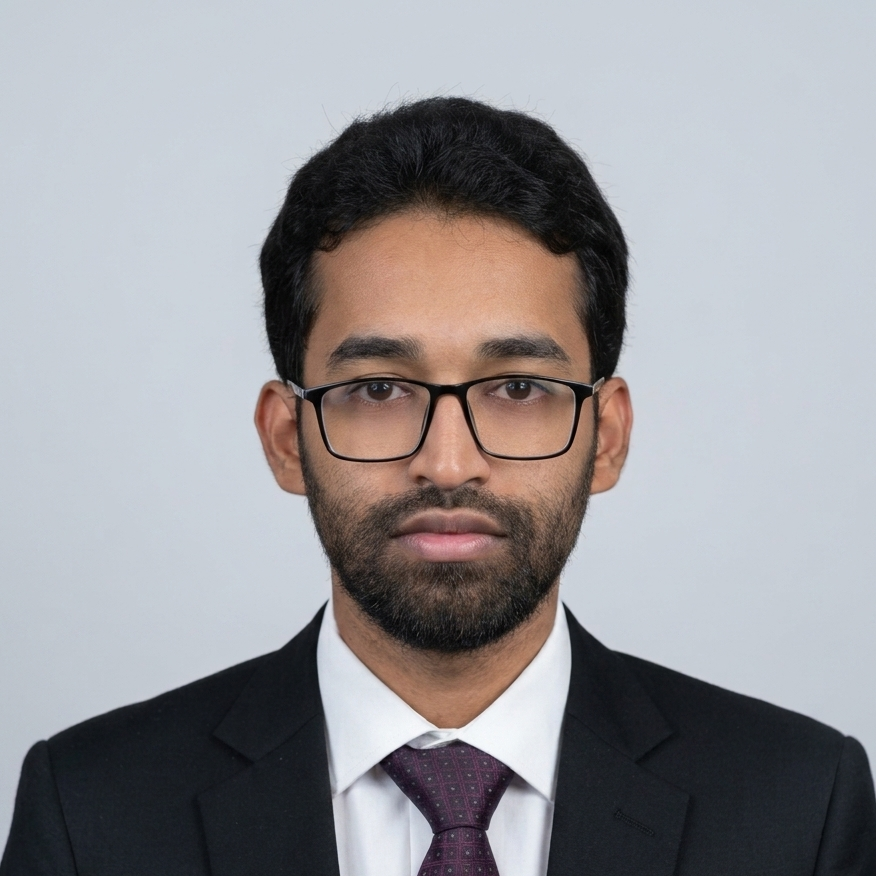
\includegraphics[width=2.5cm, height=2.5cm,
      keepaspectratio]{profile_photo.png}}; % Replace with your filename
    \end{tikzpicture}
  \end{tabularx}
\end{header}

\vspace{5 pt - 0.3 cm}

% --------------------------- Career Objective -----------------------------

\section{Career Objective}

\justifying
% \begin{onecolentry}
%   I am an aspirant engineer who wants to solve the problems found in local
%   and international energy sectors with the help of my knowledge in
%   energy engineering. I see myself as a life long learner and it is my
%   hobby to learn about new things in science and also in humanities.
% \end{onecolentry}

% \begin{onecolentry}
%   I am an aspiring engineer dedicated to addressing challenges in
% local and international energy sectors using my expertise in energy
% engineering. I view myself as a lifelong learner, with a passion
% for exploring new developments in science and humanities.
% \end{onecolentry}

\begin{onecolentry}
  I am an aspiring engineer committed to tackling challenges in local and
  international energy sectors using my expertise in energy engineering. I
  view myself as a lifelong learner, with a keen interest in advancing my
  knowledge of science, technology, and innovative engineering solutions.
\end{onecolentry}

% ------------------------------- Education -----------------------------------

\section{Education}

\begin{twocolentry}{
    2022 – 2026
  }
  \textbf{Khulna University of Engineering \& Technology},
  Khulna-9203, Bangladesh
\end{twocolentry}

\begin{onecolentry}
  B.Sc. in Energy Science and Engineering | CGPA 2.80/4.00 \\
  Coursework: Thermodynamics | Fluid Mechanics | Heat and Mass
  Transfer | Power Plant Engineering | Renewable Energy Engineering
  | IC Engines | HVAC\&R | Engineering Drawing and Simulation |
  Electrical Fundamentals
\end{onecolentry}

\vspace{0.1 cm}

\begin{twocolentry}{
    2018 – 2021
  }
  \textbf{Govt. Science College}, Tejgaon, Dhaka-1215\\
  Higher Secondary Certificate | GPA 5.00/5.00
\end{twocolentry}

\vspace{0.1 cm}

\begin{twocolentry}{
    2018
  }
  \textbf{Bright School and College}, Donia, Dhaka-1236\\
  Secondary School Certificate | GPA 5.00/5.00
\end{twocolentry}

% -------------------------------- Experience ----------------------------------

\section{Professional Experience \& Workshops}

\begin{onecolentry}
  \textbf{Industrial Attachment}, Karnaphuli Power Ltd, Chattogram
  \hfill
  Sep 2024

  \begin{highlightsforbulletentries}
    % \item Completed training on steam and diesel power plant
    %   operation and their key components and subsystems.
  \item Gained hands‑on experience operating steam and diesel
    power‑plant components, mastering key subsystems.
  \end{highlightsforbulletentries}
\end{onecolentry}

% \begin{twocolentry}{
%     May 2024
% }
%   \textbf{Training on Occupational Safety, Health \& Environment\\
%   Management}\\ Department of Energy Science and Engineering, Khulna
%   University of Engineering \& Technology, Khulna-9203, Bangladesh
% \end{twocolentry}

\begin{onecolentry}
  \textbf{Training on Occupational Safety, Health \& Environment
  Management} \hfill May 2024 \\ Department of Energy Science and
  Engineering, Khulna
  University of Engineering \& Technology

  \begin{highlightsforbulletentries}
    % \item Mastered about hazard identification, different risk analysis
    %   methods and effective environment management strategies for
    %   occupational safety.
  \item Conducted hazard identification and applied risk‑analysis
    methods to improve occupational safety management.
  \end{highlightsforbulletentries}
\end{onecolentry}

% \vspace{0.2 cm}

% \begin{twocolentry}{
%   February 2024
% }
%   \textbf{Wrokshop on Crafting Innovation: Bridging Entrepreneurship and
%   Hardware Projects in the Fab Lab Ecosystem}, FabLab, Khulna University of
%   Engineering \& Technology, Khulna-9203, Bangladesh
% \end{twocolentry}
%
% \vspace{0.10 cm}
% \begin{onecolentry}
%   \begin{highlights}
%     \item Learned about different manufacturing process, e.g., additive,
%       subtractive
%     \item Learned about different buisness models for utilizing
%       manufacturing techniques for a successful business
%   \end{highlights}
% \end{onecolentry}
%
%
% \vspace{0.2 cm}
%
% \begin{twocolentry}{
%   February 2024
% }
%   \textbf{Industrial Visit in HAMKO}, FabLab, Khulna University of
%   Engineering \& Technology, Khulna-9203, Bangladesh
% \end{twocolentry}
%
% \vspace{0.10 cm}
% \begin{onecolentry}
%   \begin{highlights}
%     \item
%     \item
%   \end{highlights}
% \end{onecolentry}
%
%
% \vspace{0.2 cm}
%
% \begin{twocolentry}{
%   February 2024
% }
%   \textbf{Industrial Visit in Atomic Energy Research Establishment}, Dhaka
% \end{twocolentry}
%
% \vspace{0.10 cm}
% \begin{onecolentry}
%   \begin{highlights}
%     \item
%     \item
%   \end{highlights}
% \end{onecolentry}

% ------------------------------ Projects --------------------------------------

\section{Research \& Project Experience}

\begin{onecolentry}
  \textbf {Energy, Exergy, and Exergoeconomic Optimization of Vapor Compression
  Refrigeration Cycle Using Low GWP Refrigerants}, Undergraduate Thesis

  \begin{highlightsforbulletentries}
  \item Investigated the effects of condensation and evaporation
    temperatures on key thermodynamic and exergoeconomic parameters
    (e.g., COP, operating cost) for basic and two-stage vapor
    compression refrigeration cycles, achieving an average
    improvement of 32\% in COP and 24\% in exergetic efficiency across
    multiple refrigerants.
    % \item Compared basic and multistage
    % VCRC performance across four
    %   low-GWP refrigerants over full evaporation/condensation ranges,
    %   uncovering a cycle-dependent crossover where R1233ZDE overtakes
    %   hydrocarbon refrigerants in COP and exergetic efficiency once staged
    % \item Optimized refrigerant-cycle combinations via entropy-weighted
    %   multi-criteria analysis, identifying multistage R1233ZDE as
    %   achieving the highest COP (3.278) and exergetic efficiency
    %   (0.766) among all fluids at a lower cost than both hydrocarbons
  \end{highlightsforbulletentries}
\end{onecolentry}

\begin{onecolentry}
  \textbf{Automated Water Level Controlling Using ESP32 and Micropython},
  3\textsuperscript{rd} Year 2\textsuperscript{nd} Term Project

  \begin{highlightsforbulletentries}
  \item Designed a real-time automated water reservoir monitoring
    system using an ESP32 microcontroller and MicroPython, reducing
    manual oversight and optimizing pump runtime cycles.
  \end{highlightsforbulletentries}
\end{onecolentry}

% -------------------------------- Skills --------------------------------------

\section{Skills}

\begin{onecolentry}
  \textbf{Engineering Tools \& Software:} CAD (SolidWorks, FreeCAD),
  MATLAB, \LaTeX, Linux Environment
\end{onecolentry}

\begin{onecolentry}
  \textbf{Technical \& Data Analysis:} Engineering Computation
  (NumPy, SciPy, SymPy), Data Visualization (Matplotlib), Predictive
  Modeling (Python), Thermodynamic Analysis (Energy, Exergy, Exergoeconomic)
\end{onecolentry}

% \begin{onecolentry}
%   \textbf{Core Competencies:} Mechanical Inspection, Thermal Systems
%   Troubleshooting, Maintenance Planning Support, Technical Documentation
% \end{onecolentry}

% ----------------- Extracurricular Activities ---------------------------------

\section{Extracurricular Activities \& Achievements}

\begin{onecolentry}
  \begin{highlightsforbulletentries}
  \item Achieved First Runner-up position in Poster Presentation
    segment at Energy Fest 1.0.
  \item Acquired management experience as Treasurer at Energy and
    Automation Club.
  \item
    \href{https://www.worldcubeassociation.org/persons/2025ROHA01}{Secured
      an average time of 18.89 s in 3x3x3 Rubik's Cube segment at
    KUET MSE Cube Rush 2025.}
    % \item Participated in Intra KUET Programming Contest
  \end{highlightsforbulletentries}
\end{onecolentry}

% -------------------------------- References ----------------------------------

\section{References}

% \begin{twocolentry}{
%     Ali Kamal Mostofa Rubel \\
%     Safety Analyst \\
%     \href{https://www.nirapon.org/}{Nirapon Inc.} \\
%     9\textsuperscript{th} Floor, Concord MB Tower,
%     House-81, Road-11, Banani,
%     Dhaka-1213, Bangladesh \\
%     Phone: \mbox{\hrefWithoutArrow{tel:+8801682560119}{01682-560119}} \\
%     Email:
%     \hrefWithoutArrow{mailto:alikamal.rubel@nirapon.org}{alikamal.rubel@nirapon.org}
%   }
%   Mostafizur Rahaman \\
%   Assistant Professor \\
%   Department of Energy Science and Engineering \\
%   Khulna University of Engineering \& Technology \\
%   Khulna-9203, Bangladesh \\
%   Phone: \mbox{\hrefWithoutArrow{tel:+8801903767842}{01903-767842}} \\
%   E-mail:
%   \hrefWithoutArrow{mailto:mostafiz@ese.kuet.ac.bd}{mostafiz@ese.kuet.ac.bd}
% \end{twocolentry}

\begin{onecolentry}
  \begin{minipage}[t]{0.48\textwidth}
    \href{https://kuet.ac.bd/ese/mostafiz}{Mostafizur Rahaman} \\
    Assistant Professor \\
    Department of Energy Science and Engineering\\
    Khulna University of Engineering \& Technology \\
    % Khulna-9203, Bangladesh \\
    Phone: \hrefWithoutArrow{tel:+8801903767842}{01903-767842} \\
    Email:
    \hrefWithoutArrow{mailto:mostafiz@ese.kuet.ac.bd}{mostafiz@ese.kuet.ac.bd}
  \end{minipage}
  \hfill
  \begin{minipage}[t]{0.48\textwidth}
    \raggedleft
    Ali Kamal Mostofa Rubel \\
    Safety Analyst \\
    \href{https://www.nirapon.org/}{Nirapon Inc.} \\
    % 9\textsuperscript{th} Floor, Concord MB Tower,
    % House-81, Road-11,
    Banani, Dhaka-1213, Bangladesh \\
    Phone: \hrefWithoutArrow{tel:+8801682560119}{01682-560119} \\
    Email:
    \hrefWithoutArrow{mailto:alikamal.rubel@nirapon.org}{alikamal.rubel@nirapon.org}
  \end{minipage}%
\end{onecolentry}

\end{document}
